\documentclass[12pt]{article}
\usepackage[margin=1in, headheight=20pt]{geometry}
\usepackage{xcolor}
\usepackage{tikz}
\usepackage{eso-pic}
\usepackage{amsthm, amsmath, amssymb}
\usepackage{mathtools}
\usepackage[italicdiff]{physics}
\usepackage{enumitem}
\usepackage{lmodern}
\usepackage{fancyhdr}
\usepackage{pgfornament}
\usepackage{parskip}
\usepackage{verbatim}

\definecolor{pagecolor}{HTML}{DCE2F0}
\definecolor{textcolor}{HTML}{373D4A}

\pagecolor{pagecolor}
\color{textcolor}

\AddToShipoutPictureBG{
  \begin{tikzpicture}[remember picture, overlay]
    \draw[
      line width=0.5pt,
      color=textcolor,
      opacity=0.075
    ]
    (current page.south west) grid[step=10pt] (current page.north east);
  \end{tikzpicture}
}

\pagestyle{fancy}
\fancyhf{}
\fancyhead[L]{Algebra I}
\fancyhead[R]{Tutorial Sheet 1}
\fancyfoot[C]{}

\renewcommand{\headrule}{
  \vspace{-5pt}
  \hbox to \headwidth{
    \leaders\hrule height 0.5pt\hfill
    \hspace{5pt}
    \raisebox{0.20pt}{\pgfornament[width=1cm]{11}}
    \hspace{5pt}
    \leaders\hrule height 0.5pt\hfill
  }
}

\renewcommand{\footrule}{
  \vspace{-12pt}
  \hbox to \headwidth{
    \leaders\hrule height 3.5pt depth -3pt \hfill 
    \hspace{5pt} 
    \thepage 
    \hspace{5pt}
    \leaders\hrule height 3.5pt depth -3pt \hfill
  }
}

\fancypagestyle{plain}{
  \fancyhf{}
  \renewcommand{\headrulewidth}{0pt}
  \renewcommand{\headrule}{} 
  \fancyfoot[C]{}
  \renewcommand{\footrule}{
    \vspace{-12pt}
    \hbox to \headwidth{
      \rule[0.65ex]{0.47\headwidth}{0.5pt}%
      \hfill
      \thepage
      \hfill
      \rule[0.65ex]{0.47\headwidth}{0.5pt}%
    }
  }
}

\newcommand{\bb}[1]{\mathbb{#1}}
\newcommand{\cl}[1]{\mathcal{#1}}

\newcommand{\p}[1]{\left ( #1 \right )}
\newcommand{\bk}[1]{\left [ #1 \right ]}
\newcommand{\br}[1]{\left \{ #1 \right\}}
\newcommand{\ab}[1]{\langle #1 \rangle}

\newcommand{\f}[2]{\frac{#1}{#2}}
\newcommand{\nset}{\varnothing}
\newcommand{\oo}{\infty}
\DeclareMathOperator{\ord}{ord}

\newcommand{\gm}{\gamma}
\newcommand{\de}{\delta}
\newcommand{\De}{\Delta}
\newcommand{\ep}{\varepsilon}
\newcommand{\la}{\lambda}
\newcommand{\si}{\sigma}
\newcommand{\om}{\omega}
\newcommand{\Om}{\Omega}

\newcommand{\imp}{\Rightarrow}
\newcommand{\pmi}{\Leftarrow}
\renewcommand{\iff}{\Leftrightarrow}
\newcommand{\ffi}{\Rightarrow\!\Leftarrow}

\title{
    \textbf{Algebra I} \\
    \textbf{Solutions to Tutorial Sheet 1}
}
\author{
  Dhyan Laad \\
  \texttt{2024ADPS0875G}
}
\date{}

\begin{document}

\maketitle

\begin{enumerate}
    \item To find all finite subgroups of $\bb R^*$, we must find all elements with a finite order. If a subgroup $H$ is finite, all ements $x \in H$ must satisfy $x^n = 1$ for some $n \in \bb N$.
    \[x^n = 1 \imp x = 1, -1.\]
    As such, the only finite subgroups of $\bb R^*$ are $\{1\}$ and $\{1, -1\}$.

    \item $\ord(a^d) = n/(n, d) = n/d$.
    
    \item The six cyclic subgroups of $U(15)$ are:
    \begin{enumerate}[label=(\alph*)]
        \item $\{1\}$,
        \item $\{1, 4\}$,
        \item $\{1, 11\}$,
        \item $\{1, 14\}$,
        \item $\{1, 2, 4, 8\}$, and
        \item $\{1, 4, 7, 13\}$.
    \end{enumerate}

    \item \begin{proof}
        Every element $x$ in $G$ either has an inverse that is distinct from itself ($x \neq x^{-1}$), or is its own inverse ($x = x^{-1} \imp x^2 = e \imp \ord(x) = 2$). Let the number of elements that have an inverse distinct from itself be $k$, and the set of elements that are their own inverses be $S$. Then,
        \[\ord(G) = \abs{S} + 2k \imp \abs{S} = \ord(G) - 2k.\]
        Since $\ord(G)$ is even by hypothesis, $\abs{S}$ must also be even. Since $e^2 = e$, $e \in S$, which implies that $\abs{S} \geq 1$. But since we know that $\abs{S}$ is even, it must be the case that $\abs{S} \geq 2$. As such, there exists a nonidentity element $x \in S$ such that $x^2 = e \imp \ord(x) = 2$.
    \end{proof}

    \item Let $x \in G$ such that $\ord(x) = 3$. Then, $\ab{x} = \{e, x, x^2 = x^{-1}\}$. Note that $x \neq x^{-1}$, since that would imply that $\ord(x) = 2$. All such sets must be necessarily disjoint barring the identity element, and as such the number of subgroups of order $3$ would be
    \[\f{8}{3 - 1} = 4.\]

    \item We need only find an element $x \in U(40)$ such that $x^4 \equiv 1 \pmod{40}$ different from the identity element $1$. Consider $x = 3$: $3^4 = 81 \equiv 1 \pmod{40}$. The subgroup generated by $3$ is given by
    \[\ab{3} = \{1, 3, 9, 27\}.\]

    \item Every nonidentity element of a noncyclic group of order $4$ must have order $2$. We may test and find that $11$ and $21$ are both of order $2$. It is also necessary that the subgroup be closed under the operation: $11 \cdot 21 = 231 \equiv 31 \pmod{40}$. We require $31$ to also be of order $2$, which it is: $31^2 = 961 \equiv 1 \pmod{40}$. Therefore, our noncyclic order $4$ subgroup is
    \[\{1, 11, 21, 31\}.\]

    \item $H \not \leq (\bb C, +)$ since it is not closed under the group operation: $(2 + i) + (-1 - 5i) = 1 - 4i$.
    
    \item $H$ can be rewritten as $\{e^{it} : t \in \bb R\}$, which can be easily verified to be a group. Geometrically, these are all the points on the unit circle $\abs{z} = 1$ on the complex plane.
    
    \item \begin{enumerate}[label=(\alph*)]
        \item $\ab{8, 14} = \ab{2} = \{0, \pm 2, \pm 4, \dots\}$.
        \item $\ab{m, n} = \ab{(m, n)}$.
        \item $\ab{12, 18, 45} = \ab{3} = \{0, \pm 3, \pm 6, \dots\}$.
    \end{enumerate}

    \item \begin{proof}
        Since $G$ has more than one element, there exists a nonidentity element $x \in G$. Let $n > 1$ be the order of $x$. We know that $n$ must have atleast one prime divisor $p$, i.e. $n = pk$ for some integer $k$. We claim that $y = x^k$ has order $p$.
        \[y^p = (x^k)^p = x^{kp} = x^n = e.\]
        $y$ cannot be the identity element since then $x^k = e$, which would imply that $n \mid k$, but since $n = pk > k$, this is not possible.
    \end{proof}

    \item This proof has been omitted due to triviality.
\end{enumerate}

\end{document}